% !TeX root = ../Thesis.tex

%************************************************
\chapter{Implementation}\label{ch:implementation}
%************************************************
\glsresetall % Resets all acronyms to not used

As this work consists of modifying an existing project, implementation details, like programming language, for part of this work are fixed. It is therefore divided into three largely independent parts:

\begin{itemize}
	\item obtaining training data
	\item developing and training the \glspl{NN}
	\item integrating the \glspl{NN} into \gls{VPR}
\end{itemize}

Although the \gls{VTR} project is implemented in C++, our \glspl{NN} are implemented and trained in Python for the convenience the various data processing libraries provide, and as our selected \gls{NN} framework, \gls{tf}, is primarily available for Python. The training data generation is implemented in C++ as an extension to the \gls{VPR} Placer. 

\section{Training Data}

For supervised learning algorithms, representative training data is imperative to achieve a good fit of the target function. While it would be possible for our problem to randomly generate synthetic training data, this would generally incur a higher domain gap than real data. One reason for this would be possibly typical distributions of terminals on the grid, or the number of samples for each terminal count. Furthermore, capturing real data is easily possible, and, due to the digital nature of the domain, free of negative capturing effects.

\subsection{Generation}

Therefore, the training samples are generated by logging real temporary placements of nets occurring during placing in \gls{VPR}.

\subsubsection{Data Source}

For this, the \gls{VPR} Placer was adopted to call a logging function whenever the \gls{HPWL} is computed for some net. Then, the two benchmark circuits \textit{stereovision} and \textit{blob\_merge}, two of the larger \gls{VPR} benchmark circuits, were placed while saving the occurring net placements. This resulted in a huge number of samples from nets with a variety of terminal counts, with many samples for all small terminal counts, becoming sparse towards higher values.

One full placement run, however, produces more samples than would be practical to process, so each run was terminated once the size of the plaintext logging file reached around \SI{100}{\mega\byte}.

\subsubsection{Target Value Computation}

Our choice of the target value for the training samples, the wiring cost for wiring a net in isolation using the Maze-Router, needs to be computed from the terminal coordinates of each net placement. While the Maze-Router is already implemented in the \gls{VPR} Router, it is not sufficiently isolated to be callable for a single placed net without significant overhead.

Therefore, we implemented the Maze-Router algorithm ourselves, working with the \gls{VPR} internal data structures holding the nets and their temporary placements.

\subsection{Format}

Before logging a sample, this algorithm is called to obtain the true wiring cost we are trying to learn to predict. For each sample three lines of plaintext are written to a text file, containing all information necessary to reconstruct the relevant information about the temporary net placement:

\begin{itemize}
	\item \gls{BB} size: X and Y dimensions of the \gls{BB} of the terminal coordinates (this value is only included for convenience and could be computed from the coordinates themselves)
	\item list of relative terminal coordinates: first the source terminal, then all sink terminals in the order they are stored in \gls{VPR}; coordinates relative to the lower-left corner of the \gls{BB}
	\item target value: the wiring cost computed using the Maze-Router
\end{itemize}

\subsection{Usage}

To use these samples for training a \gls{NN}, they need to be loaded from disk again. Furthermore, an analysis of the distribution of samples over terminal counts revealed an imbalance in their distribution.

\subsubsection{Loading}

The loading of samples is done using a simple state machine looping over the lines of the text files containing the logged samples.

\subsubsection{Balancing Terminal Counts}

\begin{figure}
	\centering
	\begin{subfigure}[b]{0.45\linewidth}
		\begin{subfigure}[b]{\linewidth}
			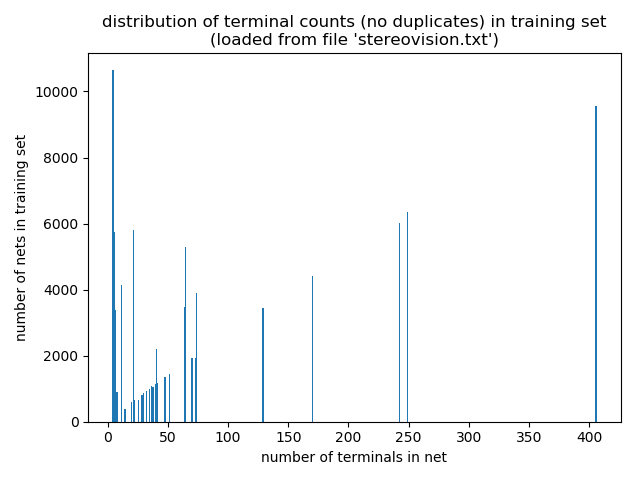
\includegraphics[width=\linewidth]{plots/data-distribution-full-fine.png}
		\end{subfigure}
		\begin{subfigure}[b]{\linewidth}
			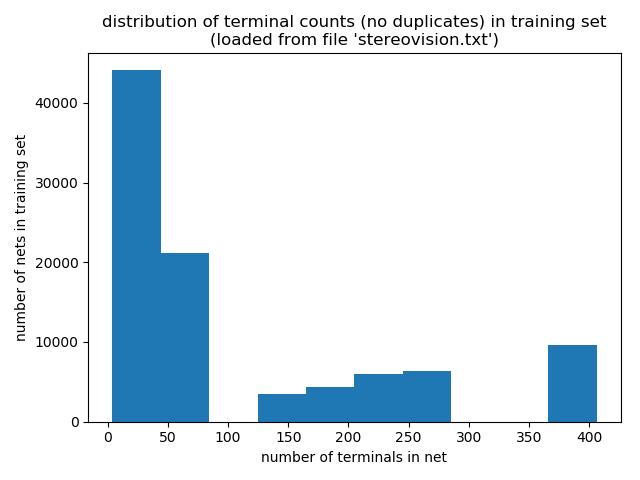
\includegraphics[width=\linewidth]{plots/data-distribution-full-coarse.png}
		\end{subfigure}
		\caption{without balancing}
	\end{subfigure}
	\begin{subfigure}[b]{0.45\linewidth}
		\begin{subfigure}[b]{\linewidth}
			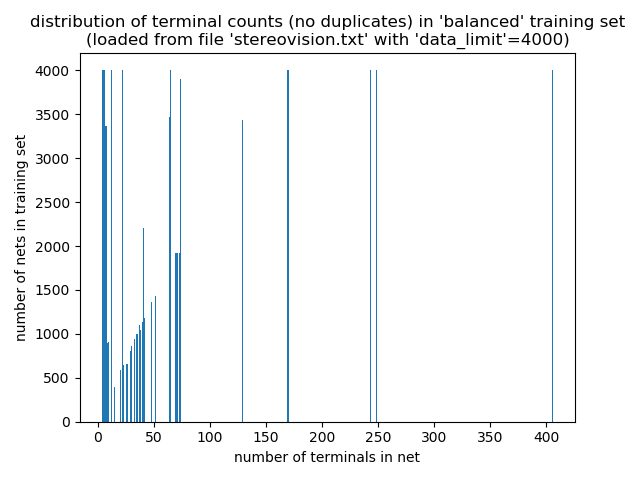
\includegraphics[width=\linewidth]{plots/data-distribution-limited-fine.png}
		\end{subfigure}
		\begin{subfigure}[b]{\linewidth}
			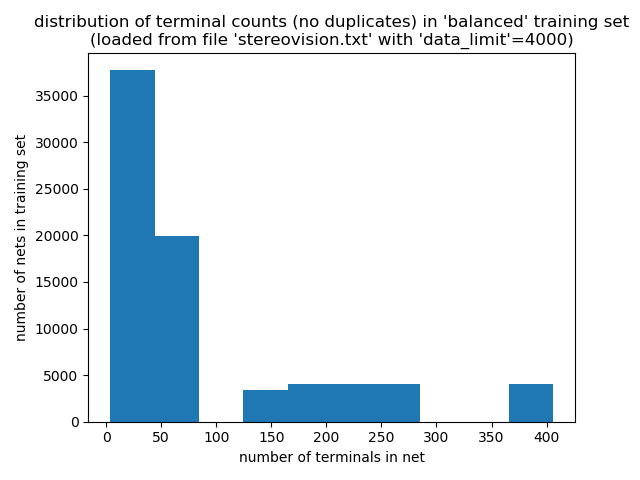
\includegraphics[width=\linewidth]{plots/data-distribution-limited-coarse.png}
		\end{subfigure}
		\caption{with balancing}
	\end{subfigure}
	\caption{Distribution of training data samples over terminal counts.}
	\label{fig:data-hist}
\end{figure}

As can be seen in \ref{fig:data-hist}, the distribution of logged training samples over the net terminal counts is not only highly sparse, but also contains very high counts at certain positions.

We decided to accept the sparsity, as it would only be avoidable with immense effort, e.g. by logging the placements of enough circuits until all counts are balanced, when using real instead of synthetic data. The \gls{NN} is expected to be able to generalize to unknown terminal counts once it is properly trained.

The imbalance on the other hand initially caused our \glspl{RNN} to notably focus on correctly predicting the cost of net placements with certain terminal counts, while neglecting the remaining samples, thereby overfitting. While this imbalance is also present in "real" data, and one could argue that this behaviour was intentional to minimize overall error, it is highly circuit specific and hinders generalization.

To that end, the samples per distinct terminal count were limited to a fixed maximum. This limit is set to 4000, which was chosen empirically to be both low enough to sufficiently balance the data, and high enough not to waste samples unnecessarily.

Our \glspl{CNN}, encoding the data in a fixed size image irrespective of terminal count, are less affected by this and were therefore trained without terminal count balancing.

\section{Neural Networks}

The \glspl{NN} themselves are implemented as \gls{tf} 2.0 Keras models, both defined and trained in a Python project.

\subsection{\gls{tf} Framework}

\gls{tf} is a \gls{ML} framework specialized in Deep Learning.\cite{tensorflow2015-whitepaper} Since its 2.0 release in 2019, it implements the Keras interface\cite{chollet2015keras}, which simplifies model definition to stacking predefined layer types, only requiring to specify input and output tensor dimensions of the full network, as well as architectural parameters, such as neuron count, per layer.

\subsection{\gls{CNN}}

The defining feature of \glspl{CNN} are their convolutional layers, mainly defined by the number and size of their filters, as well as the stride and input extension. The input is a multidimensional tensor, usually an image with one (greyscale) or three (rgb) channels.

\subsubsection{Input Format}

\begin{figure}
	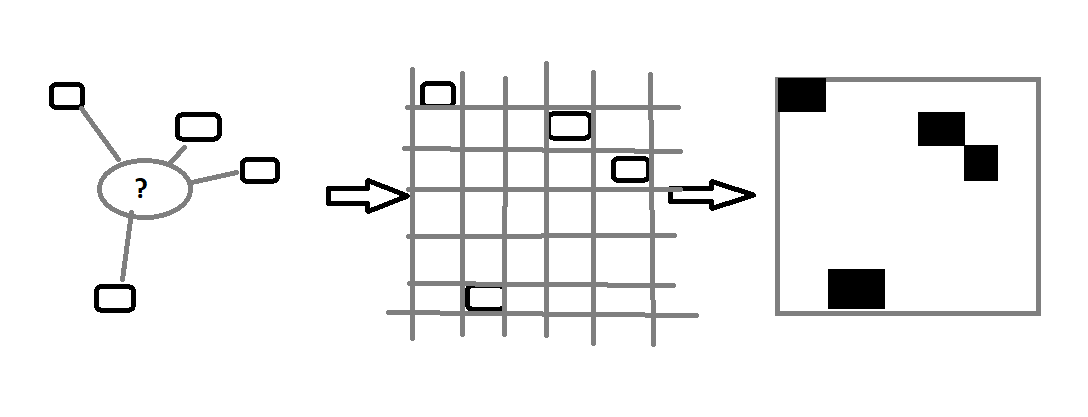
\includegraphics[width=\linewidth]{plots/cnn-encoding.png}
	\caption{Visualisation of net placement encoding procedure for \glspl{CNN}.}
	\label{fig:cnn-encoding}
\end{figure}

For our \glspl{CNN} the input coordinates have to be mapped to such an image. This is illustrated in \ref{fig:cnn-encoding}.

First, the lower-left corner of their \gls{BB} is subtracted, which is known from the remaining part of the \gls{HPWL} implementation. This helps to reduce the maximum occurring coordinates.

Next, a black image (filled with 0-valued pixels) with a fixed size of 64x64px is prepared. Now the value of the pixels at those coordinates is set to 1. This results in a binary-valued image, the lower-left corner of which directly maps to the \gls{BB} of the net placement, where all terminals which have to be connected are represented by pixels with a value of 1.

This scheme is only applicable for net placements with a \glspl{BB} not exceeding that size. However, this size was selected large enough so that all net placements occurring during the placement of the tested benchmarking circuits fit inside this limit. Indeed, the maximum \gls{BB} side length logged during training data generation is 54 units, therefore 64 units provides a certain upward margin for robustness. In the modified \gls{VPR} Placer, this limit is checked at runtime, and exceeding placements are handled by falling back to the original \gls{HPWL} computation.

By mapping coordinate values to pixel values, the sample inputs are automatically scaled to the range [0,1], making them appropriate for processing with \glspl{NN}.

The target value for each sample is the unscaled Maze-Router wiring cost, as this saves the effort of post-processing the output in the runtime-critical integration into \gls{VPR}.

\subsubsection{Structure}\label{ch:cnn-design}

\begin{figure}
	\centering
	\begin{subfigure}[b]{0.3\linewidth}
		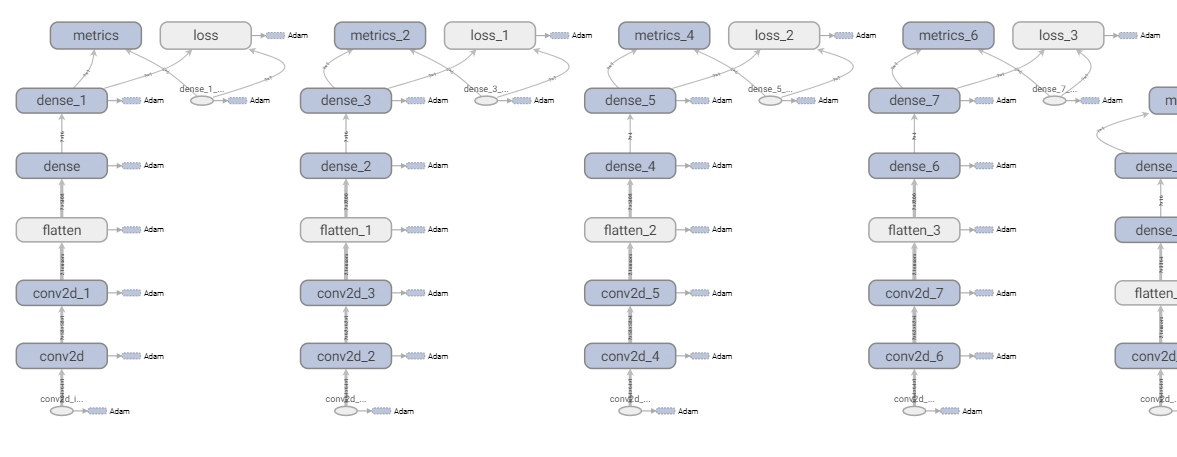
\includegraphics[width=\linewidth]{plots/cnn-candidates-2-conv.png}
		\caption{2 conv layers}
	\end{subfigure}
	\begin{subfigure}[b]{0.3\linewidth}
		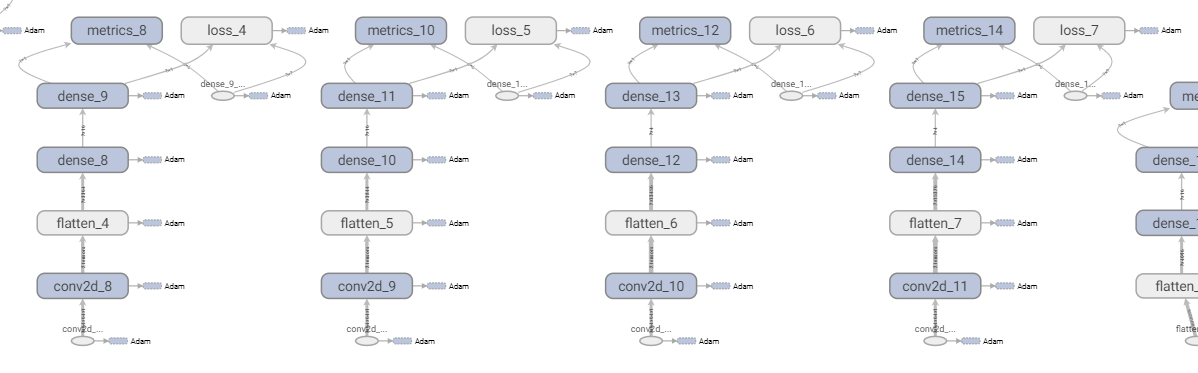
\includegraphics[width=\linewidth]{plots/cnn-candidates-1-conv.png}
		\caption{1 conv layer}
	\end{subfigure}
	\begin{subfigure}[b]{0.3\linewidth}
		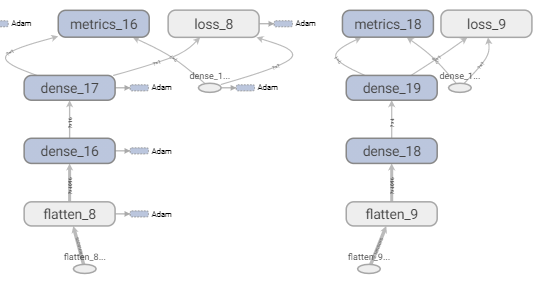
\includegraphics[width=\linewidth]{plots/cnn-candidates-0-conv.png}
		\caption{0 conv layers}
	\end{subfigure}
	\caption{Graph structures of \gls{CNN} candidates.}
	\label{fig:cnn-structure-abstract}
\end{figure}

To keep runtime small, the structure of our \glspl{CNN} is kept simple, with only few and small layers.

Our general \gls{CNN} design, as illustrated in \ref{fig:cnn-structure-abstract}, consists of zero to two convolutional layers, followed by a flatten and one to two dense layers. As the last layer, however, is always a dense layer with a single neuron, to achieve regression of one target variable, and the flatten layer is parameter-less, this leaves one to three custom layers. 

The special case of zero convolutional layers reduces the network to a plain artificial \gls{NN}, consisting only of dense layers and one flatten layer, which does not perform any computation but only reshapes the input. As these network variants, however, use the same encoding, and thus the same pre- and post-processing, they are treated the same as the remaining \glspl{CNN}.

The neuron counts per dense layer are structured by two patterns, either with counts increasing to 16 neurons for the last hidden layer, or decreasing to 4.

The filter size of the convolutional layers can be 3x3 or 7x7, but is constant within all convolutional layers of a specific network.

\subsubsection{Training}

\begin{figure}
	\centering
	\begin{subfigure}[b]{0.3\linewidth}
		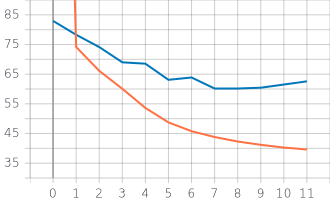
\includegraphics[width=\linewidth]{plots/cnn-training-history-2_conv_layers_deflating_kernel_size_7.png}
		\caption{2 conv layers}
	\end{subfigure}
	\begin{subfigure}[b]{0.3\linewidth}
		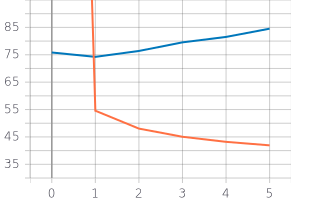
\includegraphics[width=\linewidth]{plots/cnn-training-history-1_conv_layers_deflating_kernel_size_7.png}
		\caption{1 conv layer}
	\end{subfigure}
	\begin{subfigure}[b]{0.3\linewidth}
		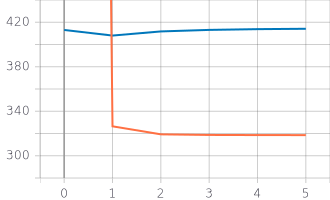
\includegraphics[width=\linewidth]{plots/cnn-training-history-0_conv_layers_deflating_kernel_size_-1.png}
		\caption{0 conv layers}
	\end{subfigure}
	\caption{Exemplary training histories (training (red) and evaluation (blue) error over epochs) of \gls{CNN} candidates with different complexity.}
	\label{fig:cnn-train}
\end{figure}

For this network, we use the standard training loop by calling the \textit{fit(...)} method of the \gls{tf} model, specifying training and validation data as well as number of epochs and batch size.

However, as using images to represent coordinates is an extremely inefficient encoding, and we have many samples, it is not possible with our available hardware to hold the full set of training data in memory. Therefore, we prepared the samples as \textit{tfrecord} files stored on disk, each holding 1.000 samples, and pass a generator to the fit method instead of the actual samples.

This generator (a slightly adapted version of the one used in a public project\cite{tfrecord-project-web}) pre-loads several such files and shuffles the samples both externally and internally for a randomized ordering. This significantly reduces memory usage during training, but introduces an additional bottleneck, which causes the CPU utilization to drop.

Furthermore, in order to keep the effort of training all \gls{CNN} candidates manageable, the dataset was artificially limited to 200.000 samples.

The performance is logged using TensorBoard\cite{tensorboard-web}, and in the end the trained model is saved in the \gls{tf} SavedModel format\cite{savedmodel-web}, ready to be deployed to our adapted version of \gls{VPR}.

Early stopping, with a patience of 4, and checkpointing are deployed to automatically detect overfitting and save only the best weights evaluated during training of each model. This is necessary as the model might start to overfit or lose performance due to the inoptimality of the stochastic gradient descent used to train the model. Indeed, our \gls{CNN} models tend to overfit quickly, depending on the model complexity (see \ref{fig:cnn-train}). 

\subsection{\gls{RNN}}

\glspl{RNN} are defined by the presence of recurrent layers, which feed some information back to their input, establishing a state in the prediction operation. This state allows them to remember former inputs and thus to process sequences instead of only single tensors. Thus they can process inputs of variable size, typically with one not strictly defined input dimension.

\subsubsection{Input Format}

\begin{figure}
	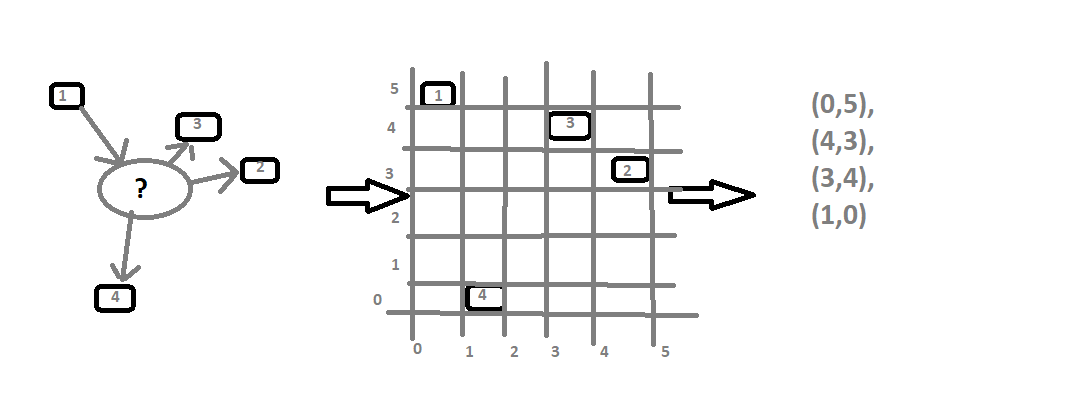
\includegraphics[width=\linewidth]{plots/rnn-encoding.png}
	\caption{Visualisation of net placement encoding procedure for \glspl{RNN}.}
	\label{fig:rnn-encoding}
\end{figure}

As the \gls{RNN} accepts sequences of variable length as input data, we encode the terminal positions as a ordered list of coordinate pairs, as shown in \ref{fig:rnn-encoding}.

To support efficient training we scale our training data. As the distribution of the terminals inside their \gls{BB} is approximately uniform (based on the properties of the simulated annealing placer), we normalize the coordinates to the range [0,1] by dividing by the maximum of their \glspl{BB}' X and Y dimensions. 

In the Maze-Router, all distances are computed using the Manhattan metric, and the result of the algorithm is a linear combination of distances. Therefore, linear scaling of the input values does not require recomputing the expected result, as the original result can simply be scaled using the same factor used when scaling the inputs.

As the scaling factor itself is not part of the input to the \gls{RNN}, it can only learn to predict the result of the scaled problem. Therefore, we need to post process the predicted output in our adapted \gls{VPR} implementation by rescaling it to the original magnitude using the inverse of the scaling factor of the inputs.

\subsubsection{Structure}\label{ch:rnn-design}



\begin{figure}
	\centering
	\begin{subfigure}[b]{0.3\linewidth}
		\begin{subfigure}[b]{\linewidth}
			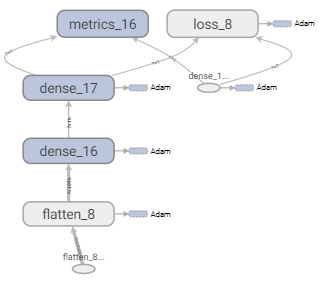
\includegraphics[width=\linewidth]{plots/rnn-candidates-placeholder.png}
		\end{subfigure}
		\begin{subfigure}[b]{\linewidth}
			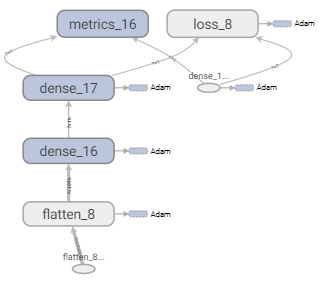
\includegraphics[width=\linewidth]{plots/rnn-candidates-placeholder.png}
		\end{subfigure}
		\caption{3 lstm layers}
	\end{subfigure}
	\begin{subfigure}[b]{0.3\linewidth}
		\begin{subfigure}[b]{\linewidth}
			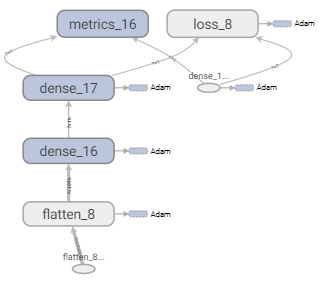
\includegraphics[width=\linewidth]{plots/rnn-candidates-placeholder.png}
		\end{subfigure}
		\begin{subfigure}[b]{\linewidth}
			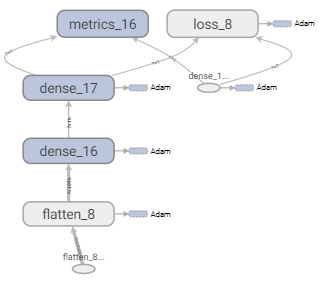
\includegraphics[width=\linewidth]{plots/rnn-candidates-placeholder.png}
		\end{subfigure}
		\caption{2 lstm layers}
	\end{subfigure}
	\begin{subfigure}[b]{0.3\linewidth}
		\begin{subfigure}[b]{\linewidth}
			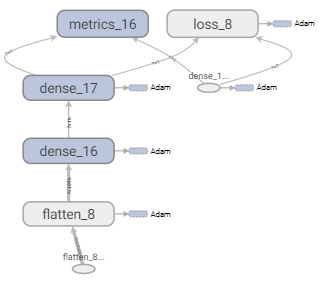
\includegraphics[width=\linewidth]{plots/rnn-candidates-placeholder.png}
		\end{subfigure}
		\begin{subfigure}[b]{\linewidth}
			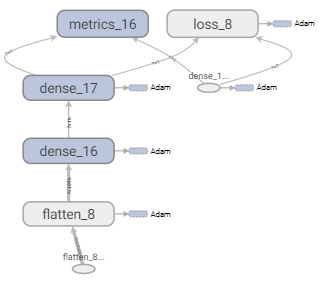
\includegraphics[width=\linewidth]{plots/rnn-candidates-placeholder.png}
		\end{subfigure}
		\caption{1 lstm layer}
	\end{subfigure}
	\caption{Graph structures of \gls{RNN} candidates (TODO placeholders...).}
	\label{fig:rnn-structure-abstract}
\end{figure}

Similarly to the \gls{CNN} structure, our \glspl{RNN} are composed of \gls{LSTM} layers followed by dense layers (see \ref{fig:rnn-structure-abstract}). However, each \gls{RNN} has to contain at least one \gls{LSTM} layer, as the last \gls{LSTM} layer encodes the variable length sequences into fixed size tensors that can be processed by the following dense layers.

Thus, one to three \gls{LSTM} layers are followed by one or two dense layers, the last dense layer again being the fixed one-neuron output layer. Here, the neuron count is specified for both dense and \gls{LSTM} layers. The three patterns \textit{increasing}, \textit{decreasing}, and \textit{bloating} control the distribution of neurons over the layers, de- or increasing in steps of 4. \textit{Bloating} describes an increasing count within the \gls{LSTM} part of the network, and decreasing in the following dense layers.

\subsubsection{Training}

\begin{figure}
	\centering
	\begin{subfigure}[b]{0.45\linewidth}
		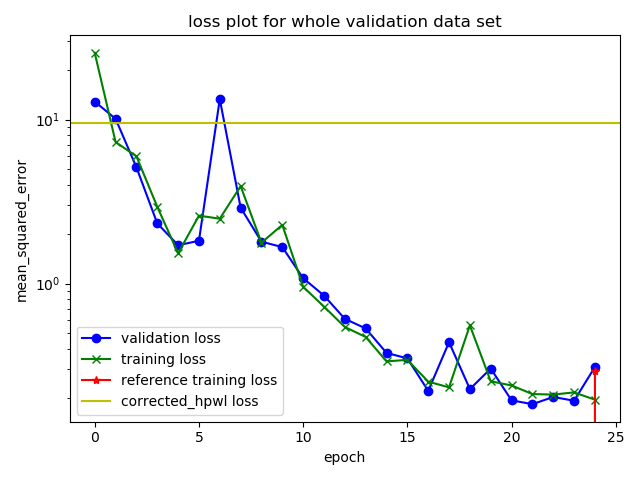
\includegraphics[width=\linewidth]{plots/rnn-training-history-3_lstm_layers_2_dense_layers_inflating.png}
		\caption{3 lstm layers, 2 dense layers}
		\label{fig:rnn-training-overfit}
	\end{subfigure}
	\begin{subfigure}[b]{0.45\linewidth}
		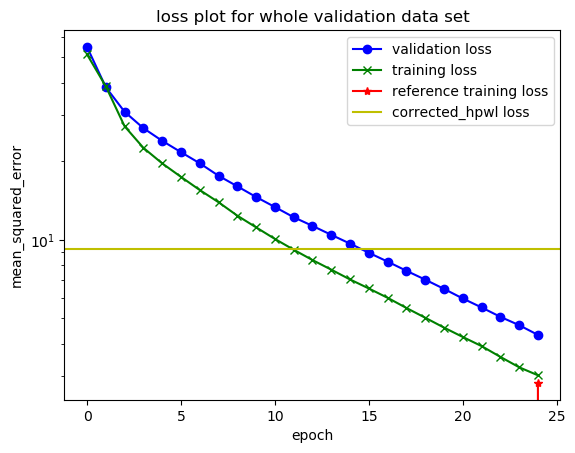
\includegraphics[width=\linewidth]{plots/rnn-training-history-1_lstm_layers_1_dense_layers_inflating.png}
		\caption{1 lstm layer, 1 dense layer}
		\label{fig:rnn-training-simple}
	\end{subfigure}
	\caption{Exemplary training histories of \gls{RNN} candidates with different complexity.}
	\label{fig:rnn-training}
\end{figure}

Although \glspl{RNN} generally support variable length input sequences, the implementation behind \gls{tf} imposes a limit on this: Input sequences within the same batch of samples are required to have uniform sequence length.

The standard \textit{fit(...)} method, however, only allows the user to specify the training data and batch size, but not to pass predefined batches.

As being able to predict the wiring cost with minimal preprocessing overhead is was the primary reason for choosing \glspl{RNN}, and a network trained only on samples padded to a common size would be unable to accurately predict on unpadded sequences, we implemented a custom training loop. This enables us to train on variably sized samples, by manually defining the batches.

Training with a batch size of 1, also called \textit{online learning}, would enable us to train on a sequence of samples with fully randomized ordering. However, this approach is generally known to not to converge to the same quality of or as stable results as minibatch learning, although being able to converge faster, i.e. on fewer samples. The runtime of the trained network, however, remains the same. As we are interested in getting as accurate predictions as possible for as little computation time as possible, and we have an abundance of training samples, we stick with minibatch learning.

For this, we model epochs by manually looping over the epoch count, and train on each batch separately using the \textit{fit()} method. We do not specify evaluation samples in the \textit{fit} calls, as the evaluation should only be done at the end of each epoch. To this end, we predict the wiring cost for each of the evaluation samples, and compute the metric score manually using the difference to the known true values.

The separation of training samples into batches is done only once in the beginning by sorting the samples by length, selecting consecutive ranges of samples with the same length as batches, and dropping the last non-full batch, if present.

To ensure a randomized order while training, we shuffle the batches both externally and internally each epoch, but we do not shuffle across batch borders for simplicity. We believe this to result in a sufficiently randomized ordering for efficient training.

Due to the custom training loop, the training of our \gls{RNN} model is not supported for supervision using TensorBoard. Therefore, we implemented simple logging and visualization to help in debugging and model selection.

\ref{fig:rnn-training} shows the training histories of two different \glspl{RNN}. While \ref{fig:rnn-training-overfit} reaches higher performance due to a higher number of trainable parameters, it does not converge as smoothly as \ref{fig:rnn-training-simple}, which, due to its simple structure, can only achieve a rough fit. The reason for the sharp spikes in both training and evaluation error can easily be explained by taking a look at \ref{fig:rnn-training-individual}. This shows the individual errors on samples of specific terminal counts. It can be observed that such a sharp drop in performance is usually caused by the model trying to lower the error on samples with high terminal counts, probably by adjusting predictions generally upwards, which causes high error on samples with low terminal counts. In the following epoch the model usually rectifies its mistake.

Another interesting observation is the fact that evaluation error frequently drops below training error, which seems to imply the model is better in predicting on unknown data than it is on known samples. This, however, is due to the way error computation is implemented in the \gls{tf} framework\cite{keras-faq-web}. The training error of an epoch is computed as the mean of the training error on all batches at the point they are used for training. Therefore, the error on the first batches is computed in a different network state than the error on the later batches. As the model usually improves during an epoch, this causes the training error to be higher than expected. Similarly, a decrease in overall performance might appear as overfitting due to validation error rising faster than the training error. The red bar in the \gls{RNN} training history plots shows the expected \textit{reference train error} after the last epoch.

Like our \gls{CNN}, the trained model is saved and can be deployed analogously. However, due to the custom training loop, early stopping and checkpointing are implemented explicitly, as the predefined callbacks can not be used in this scenario.

\section{Integration}

For integration of our \glspl{NN} into \gls{VPR}, which is implemented in C++, we modify the Placer in the central \textit{place.cpp} module. We implement an interface to our \glspl{NN} as an abstract class calling the \gls{NN} inference, implemented by a \gls{CNN} wrapper and a \gls{RNN} wrapper, performing model specific pre- and post-processing.

\subsection{\gls{tf} SavedModel}

The \glspl{NN} themselves are saved in the \gls{tf} SavedModel format, which faciliates portability across language bindings of the \gls{tf} framework. 
	
As the models are only used for inference, and will no longer be trained, we select not to include the optimizer in the saved model to save space.

\subsection{\gls{tf} C API}

The \gls{tf} C API provides language bindings for C++ as well as plain C. The executable code itself is loaded dynamically from the \textit{tensorflow.dll} dynamic link library.

However, it is not as well maintained as the Python library, and official releases are known often not to work. In our case, the precompiled dll was missing an entry point, so we needed to compile it from the source code. After fixing several incopatabilities and aquiring the necessary requirements, the compilation itself still took severel day, but succeeded eventually.

\subsection{Compile Time Integration into \gls{VPR} Placer}

As our modifications are located at the most performance-critical part of the \gls{VPR} Placer, we opted for compile time selection of operation mode to avoid introducing unnecessary control flow. 

We specified a compile time variable for four possible modes of operation: 

\begin{itemize}
	\item unchanged \gls{VPR}
	\item training data generation, writing all temporary net placements to a text file
	\item \gls{RNN} integration, replacing \gls{HPWL} with our \gls{RNN} interface for all nets with more than 3 terminals
	\item \gls{CNN} integration, replacing \gls{HPWL} with our \gls{CNN} interface for all nets with more than 3 terminals and placements not exceeding the hard limit
\end{itemize}
